\subsection{Kernel}

\begin{frame}{Konfiguration}{}
\begin{center}
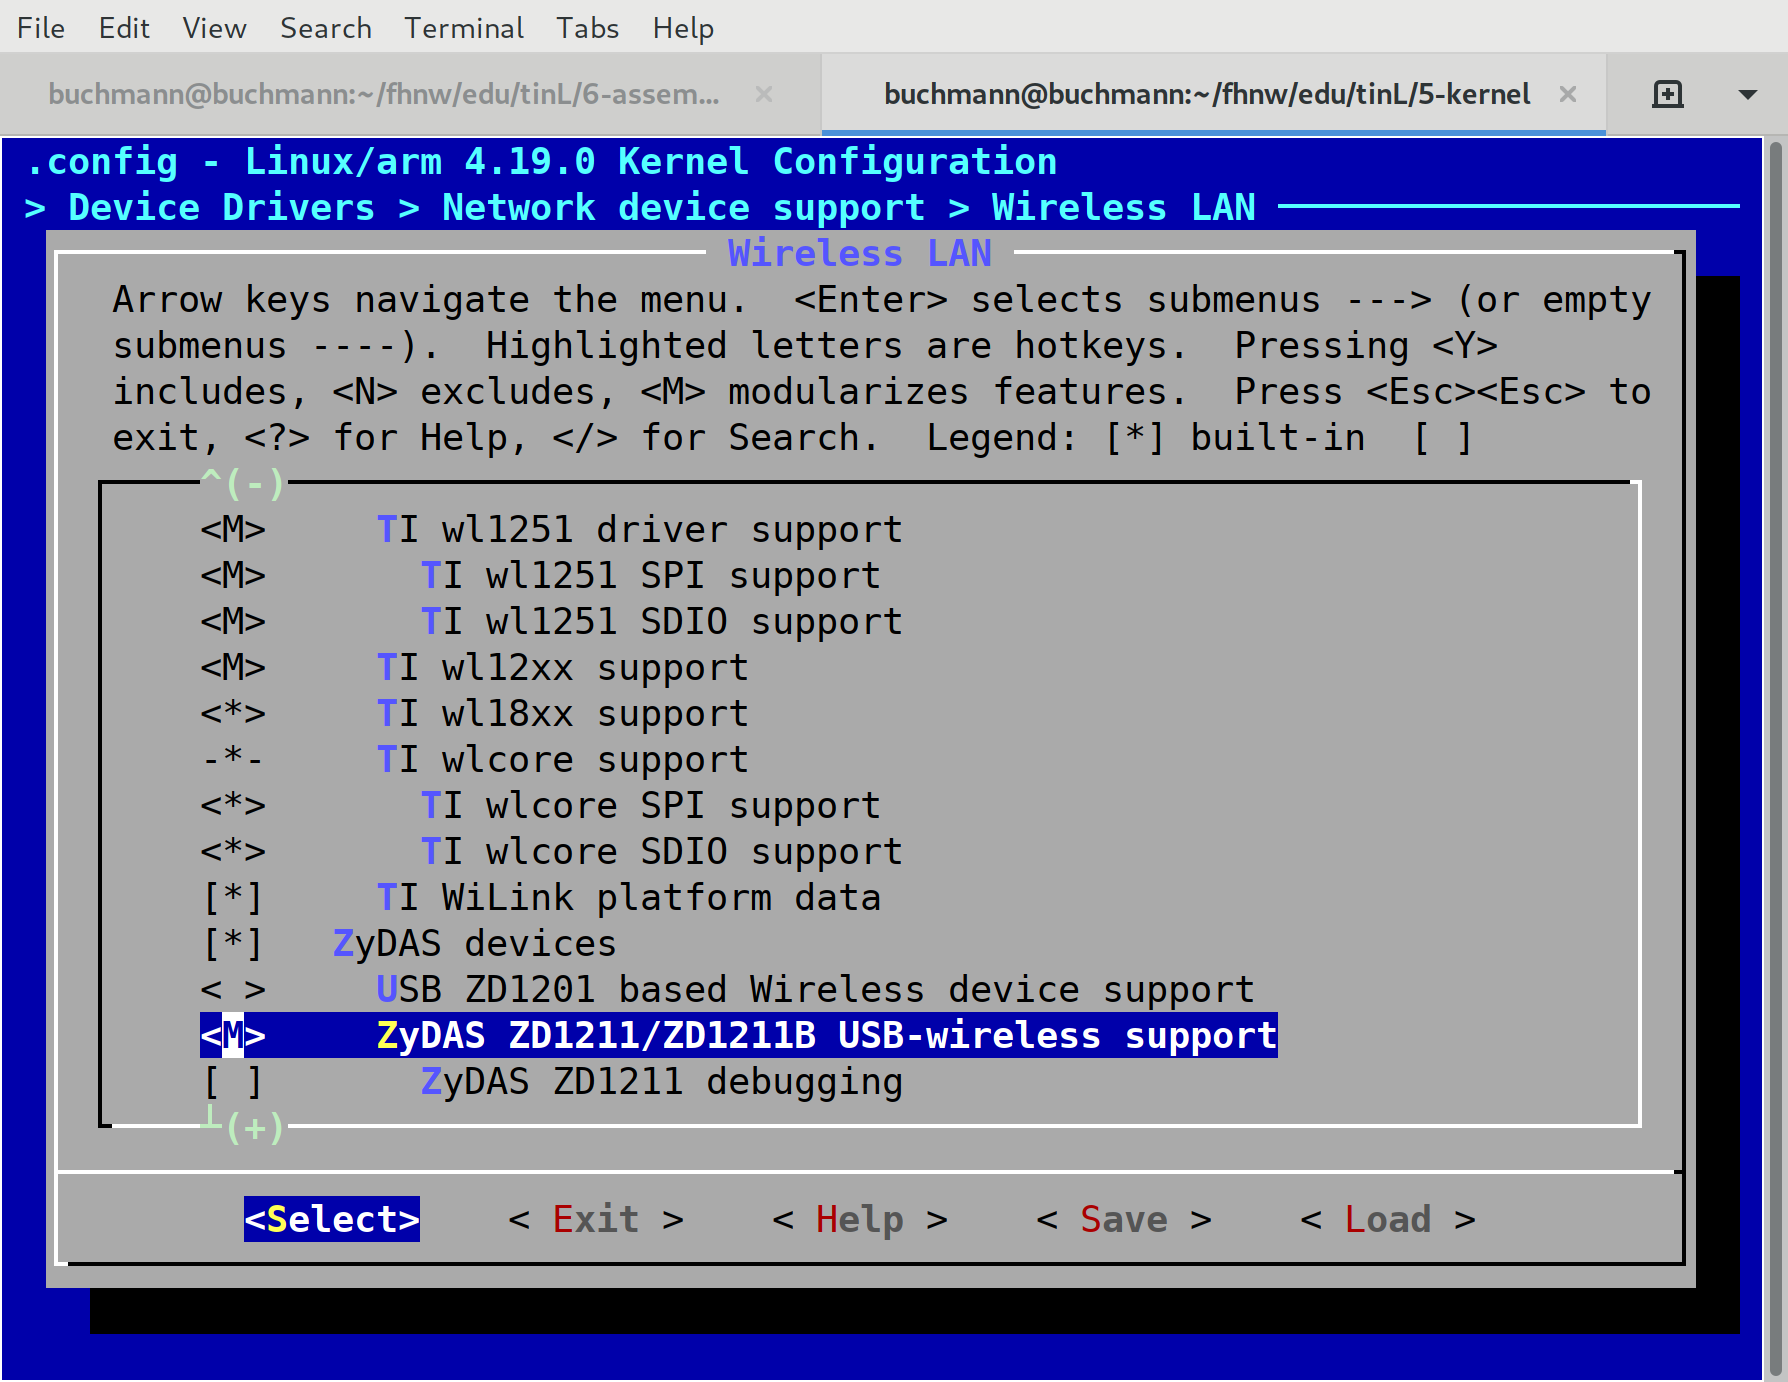
\includegraphics[height=0.75\textheight]{wl18xx.png}
\end{center}
\vspace{-2mm}
\begin{itemize}
 \item Test: \cod{dmesg | grep wl}
\end{itemize}
\end{frame}

\begin{frame}{Abh�ngigkeiten}
\begin{center}
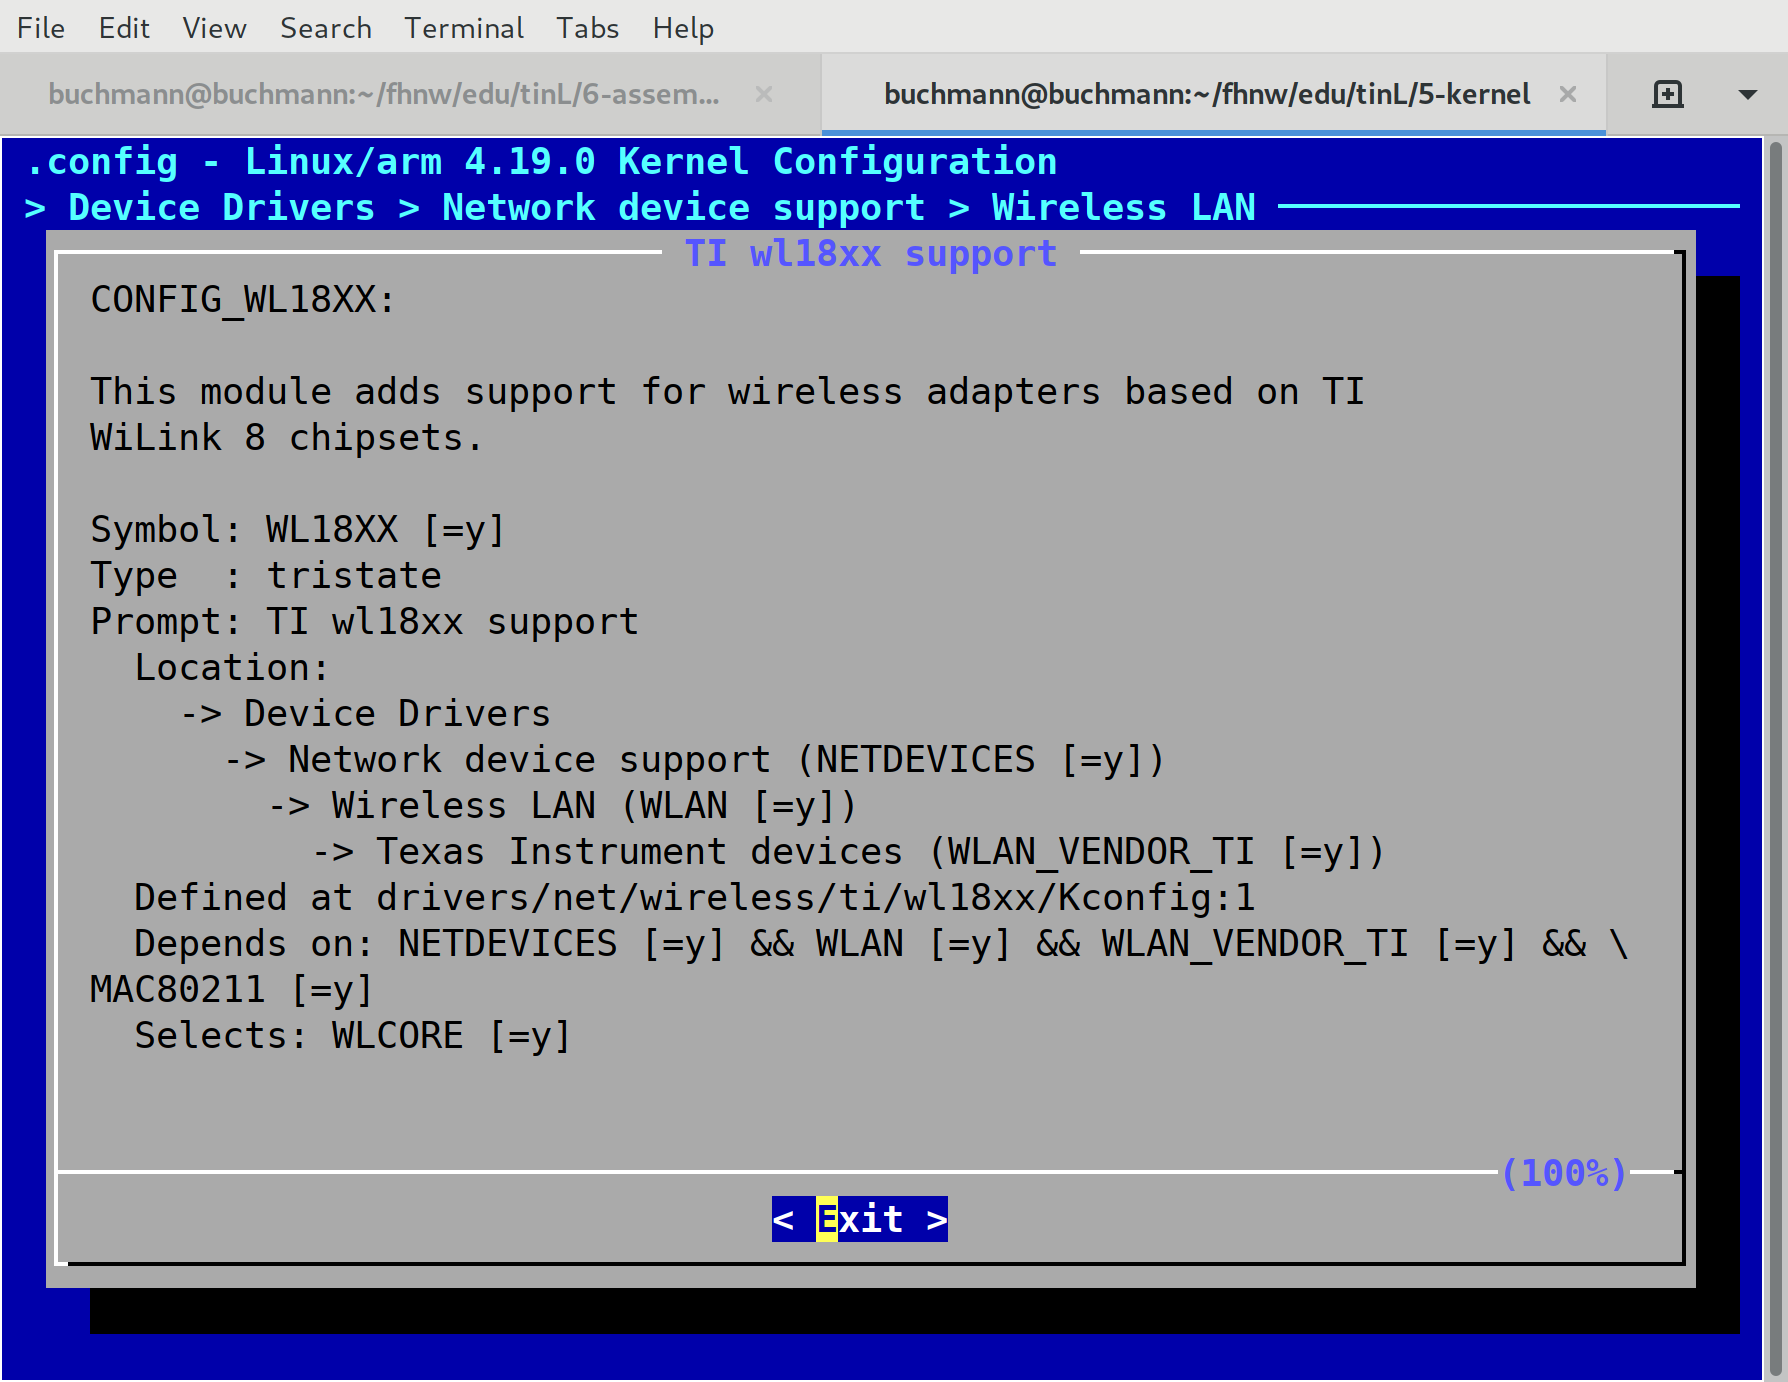
\includegraphics[height=0.75\textheight]{wl18xx-dependencies.png}
\end{center}
\end{frame}

\begin{frame}{Firmware}
\begin{center}
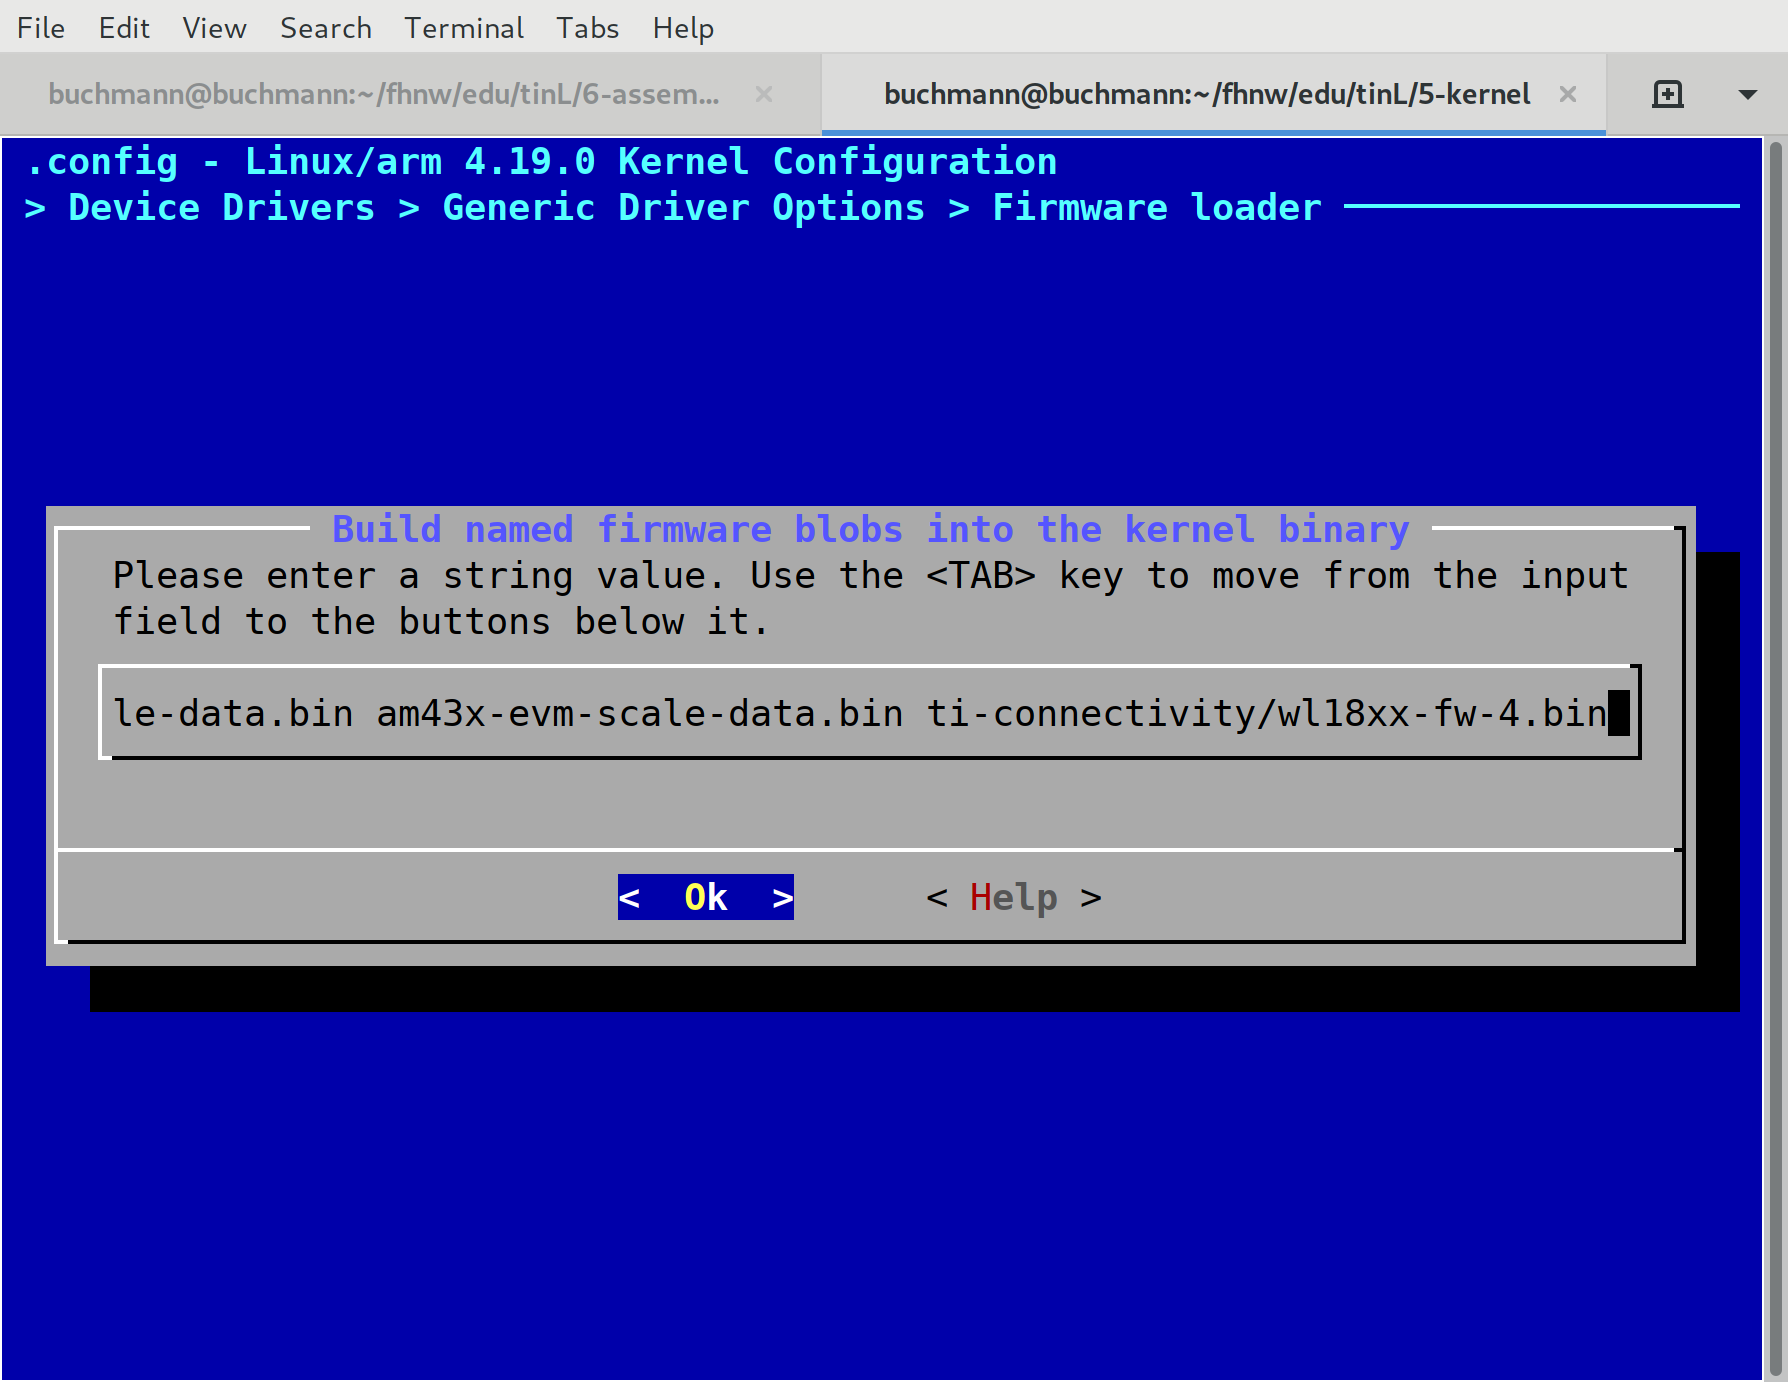
\includegraphics[height=0.75\textheight]{firmware.png}
\end{center}
\end{frame}

\begin{frame}{Test}{wlan0}
 \begin{itemize}
  \item \cod{dmesg | grep wl}
  \item \cod{ip link set wlan0 up}
  \item \cod{iw wlan0 scan}
 \end{itemize}
\end{frame}

\subsection{Connect}

\begin{frame}[fragile]{WPA}{\cod{wpa\_supplicant}, \cod{wpa}}
 \begin{itemize}
  \item Konfiguration: 
  \begin{itemize}
   \item Siehe {\em 3-network}
  \end{itemize}
  \item Process:
  \begin{itemize}
   \item \cod{wpa\_supplicant -D wext -i wlan0 -c {\em path\_to\_config}}
  \end{itemize}
  \item Bedienung (funktioniert nocch nicht)
  \begin{itemize}
   \item \cod{wpa\_cli -s {\em  wpa\_client\_socket\_file\_path}}
  \end{itemize}
 \end{itemize}
\end{frame}

\begin{frame}[fragile]{DHCP}
 \begin{block}{manuell}
  \begin{itemize}
   \item \cod{udhcpc -v -i wlan0}
   \item \cod{ifconfig wlan0 {\em ip}}
   \begin{itemize}
    \item \cod{\em ip} abgelesen von \cod{udhcpc -v -i wlan0}
   \end{itemize}
  \end{itemize}
 \end{block}
 \begin{block}{automatisch/callback}
\vspace{-3mm}
{\tiny
\begin{verbatim}
#!/bin/sh
#---------------------
#on-udhcpc.sh
#(c) H.Buchmann FHNW 2018
#---------------------
echo "-------------- on-udhcpc.sh ${1}" 
case ${1} in
 defconfig)
  echo defconfig------- ${interface} ${ip};;
  bound)
   ifconfig ${interface} ${ip};;
#set route here
esac
\end{verbatim}
}
\end{block}
\end{frame}

\begin{frame}[fragile]{route/dns}
\begin{itemize}
 \item route
 \begin{itemize}
  \item \cod{route add default gw {\em gw-ip} wlan0}
 \end{itemize}
 \item DNS
 \begin{itemize}
   \item \cod{/etc/resolv.conf:}
{\tiny
\begin{verbatim}
nameserver 147.86.4.21
#try nameserver 8.8.8.8
\end{verbatim}
 }
 \end{itemize}
 
\end{itemize}
\end{frame}

